 \documentclass[12pt,a4paper,oneside]{article}
\usepackage[spanish,es-noshorthands]{babel}
\usepackage{tikz, pgfplots, geometry, graphicx, wrapfig, tipa, circuitikz} % Entornos graficos
\usepackage{amssymb, amsmath, float, mathpazo, textcomp, gensymb, mathtools,mathrsfs} % Matematica/Simbolos
\usepackage{multicol, multirow, xcolor, colortbl}
\usepackage{lastpage, bookmark, authblk}
\usepackage{subcaption}
\usepackage{array}

% Varios
\usepackage[label=corner]{karnaugh-map}
\usepackage{threeparttable}
\usepackage{ulem, lipsum}
\usepackage{adjustbox}
\usepackage{listings}
\usepackage{fancyhdr}
\usepackage{capt-of}
\usepackage{caption}
\usepackage{cancel}
\usepackage{makecell} % Para hacer saltos de linea en tablas
\usepackage[utf8]{inputenc} % Required for inputting international characters
\usepackage[T1]{fontenc} % Output font encoding for international characters

% Librerias extra de Tikz
\pgfplotsset{compat=1.7} % !!VERSION PGF¡¡
\usetikzlibrary{patterns}
\usetikzlibrary{positioning}
\usetikzlibrary{arrows}
\usetikzlibrary{calc}
\usetikzlibrary{fpu}
\usepackage{longtable}

\definecolor{vgreen}{RGB}{104,180,104}
\definecolor{vblue}{RGB}{49,49,255}
\definecolor{vorange}{RGB}{255,143,102}
\definecolor{codegreen}{rgb}{0,0.6,0}
\definecolor{codegray}{rgb}{0.5,0.5,0.5}
\definecolor{codepurple}{rgb}{0.58,0,0.82}
\definecolor{backcolour}{rgb}{0.95,0.95,0.92}
\definecolor{mlgb}{RGB}{100,224,238}
\definecolor{mdrd}{RGB}{160,24,82}
\definecolor{mdblu}{RGB}{20,91,112}
\definecolor{mblk}{RGB}{35,35,35}


\usepackage[scr=esstix,cal=boondox]{mathalfa}
\makeatletter
\usepackage[spanish,es-noshorthands]{babel}
\usepackage{tikz, pgfplots, geometry, graphicx, wrapfig, tipa, circuitikz} % Entornos graficos
\usepackage{amssymb, amsmath, float, mathpazo, textcomp, gensymb, mathtools,mathrsfs} % Matematica/Simbolos
\usepackage{multicol, multirow, xcolor, colortbl}
\usepackage{lastpage, bookmark, authblk}
\usepackage{subcaption}
\usepackage{array}

% Varios
\usepackage[label=corner]{karnaugh-map}
\usepackage{threeparttable}
\usepackage{ulem, lipsum}
\usepackage{adjustbox}
\usepackage{listings}
\usepackage{fancyhdr}
\usepackage{capt-of}
\usepackage{caption}
\usepackage{cancel}
\usepackage{makecell} % Para hacer saltos de linea en tablas
\usepackage[utf8]{inputenc} % Required for inputting international characters
\usepackage[T1]{fontenc} % Output font encoding for international characters

% Librerias extra de Tikz
\pgfplotsset{compat=1.7} % !!VERSION PGF¡¡
\usetikzlibrary{patterns}
\usetikzlibrary{positioning}
\usetikzlibrary{arrows}
\usetikzlibrary{calc}
\usetikzlibrary{fpu}
\usepackage{longtable}

\definecolor{vgreen}{RGB}{104,180,104}
\definecolor{vblue}{RGB}{49,49,255}
\definecolor{vorange}{RGB}{255,143,102}
\definecolor{codegreen}{rgb}{0,0.6,0}
\definecolor{codegray}{rgb}{0.5,0.5,0.5}
\definecolor{codepurple}{rgb}{0.58,0,0.82}
\definecolor{backcolour}{rgb}{0.95,0.95,0.92}
\definecolor{mlgb}{RGB}{100,224,238}
\definecolor{mdrd}{RGB}{160,24,82}
\definecolor{mdblu}{RGB}{20,91,112}
\definecolor{mblk}{RGB}{35,35,35}


\usepackage[scr=esstix,cal=boondox]{mathalfa}

%Caratula
\newcommand{\subtitledoc}[1]{\newcommand{\@subtitledoc}{#1}}
\newcommand{\instituto}[1]{\newcommand{\@instituto}{#1}}
\newcommand{\carrera}[1]{\newcommand{\@carrera}{#1}}
\newcommand{\professor}[1]{\newcommand{\@professor}{#1}}
\newcommand{\catedra}[1]{\newcommand{\@catedra}{#1}}
\newcommand{\curso}[1]{\newcommand{\@curso}{#1}}
\newcommand{\legajo}[1]{\newcommand{\@legajo}{#1}}
\newcommand{\footerauthor}[1]{\newcommand{\@footerauthor}{#1}}
\newcommand{\footerlegajo}[1]{\newcommand{\@footerlegajo}{#1}}
\newcommand{\footercatedra}[1]{\newcommand{\@footercatedra}{#1}}

%Indice
\newcommand{\unsection}[1]{\addcontentsline{toc}{section}{#1}\section*{#1}}
\newcommand{\unsubsection}[1]{\addcontentsline{toc}{subsection}{#1}\subsection*{#1}}
\newcommand{\unsubsubsection}[1]{\addcontentsline{toc}{subsubsection}{#1}\subsubsection*{#1}}

%Custom
\newcommand{\longdiv}{\smash{\mkern-0.43mu\vstretch{1.31}{\hstretch{.7}{)}}\mkern-5.2mu\vstretch{1.31}{\hstretch{.7}{)}}}}
\newcommand{\lrah}{\hspace{0.25cm} \Longrightarrow \hspace{0.25cm}}
\newcommand{\llah}[1]{\hspace{0.25cm} \Longleftarrow \hspace{0.25cm}}
\newcommand{\llrah}[1]{\hspace{0.25cm} \Longleftrightarrow \hspace{0.25cm}}
\newcommand{\Real}[1]{\mathbb{R}{e}\{#1\}}
\newcommand{\Imag}[1]{\mathbb{I}{m}\{#1\}}
\newcommand{\arc}[1]{{%
    \setbox9=\hbox{#1}%
    \ooalign{\resizebox{\wd9}{\height}{\texttoptiebar{\phantom{A}}}\cr#1}}}


%Configuracion de hoja (margenes y tamaño)
\geometry{a4paper,margin=1in}
\setlength\headheight{28pt}





%Metadata para pdf
%\hypersetup{
%    pdftitle={\@title},
%    pdfsubject={\@catedra\ - \@subtitledoc},
%    pdfauthor={\@author\ - \@legajo\ - \@curso},
%    pdfkeywords={\@title\ \@catedra\ \@subtitledoc\ \@author\ \@legajo\ \@curso}
%}






%formato de encabezado y pie para todas las paginas.
\fancyhead[L]{
    \begin{minipage}[b]{7.5mm}
        
\includegraphics[width=7mm]{Imagenes/logo-utn.png}
    \end{minipage}
    \begin{minipage}[b]{100mm}
        \textbf{Alumnos: }\@footerauthor \\
        \textbf{Legajos: }\@footerlegajo
    \end{minipage}
}
\fancyhead[R]{
    \textbf{Curso:} \@curso \textbf{ - Año:} \the\year\\%/\twodigits\the\month/\twodigits\the\day\\
    \textbf{Cátedra:} \@catedra
}
\fancyfoot[C]{} %eliminar antiguo numero de pagina
\fancyfoot[R]{Página \thepage\ de \pageref{LastPage}}
\renewcommand{\headrulewidth}{0.5pt}
\renewcommand{\footrulewidth}{0.5pt}
\pagestyle{fancy}
\addto\captionsspanish{%
	\renewcommand{\contentsname}%
	{CONTENIDO}%
}

\renewcommand{\maketitle}{%
    \newpage
    \thispagestyle{empty}
    
    \begin{center}

    \textsc{\LARGE \@instituto}\\[0.5cm] 
    \textsc{\Large \@carrera}\\[1.5cm] 
    
\includegraphics[width=0.30\textwidth]{Imagenes/logo-utn.png} \par
    \vspace{0.9cm}
    
    \textsc{\large \@catedra}\\[0.85cm]
    \headrule \vspace{0.25cm}
    {\huge\bfseries \@title}\\[0.4cm]
    \textsc{\Large \@subtitledoc}\\[0.25cm]
    \headrule \vspace{0.25cm}
    
    \end{center}

    \vspace{2cm}

    {\noindent
    \begin{minipage}[t]{.2\textwidth}
        \raggedright
        \textbf{DOCENTES} \par
        \bigskip \bigskip
        \smallskip
        \textbf{CÁTEDRA} \par
        \textbf{CURSO} \par
        \medskip
        \textbf{ALUMNOS} \par
        \end{minipage}%
        \begin{minipage}[t]{.05\textwidth}
        \raggedright
        \textbf{:} \par
        \bigskip \bigskip
        \smallskip
        \textbf{:} \par
        \textbf{:} \par
        \medskip
        \textbf{:} \par
    \end{minipage}%
    \begin{minipage}[t]{.55\textwidth}
        \raggedright
        \@professor \par
        \@catedra \par
        \@curso \par
        \medskip 
        \@author \par
    \end{minipage}%
    \begin{minipage}[t]{.15\textwidth}
        \raggedright
        ~\\
        ~\\
        ~\\
        ~\\
         \bigskip \bigskip
        \@legajo \par
    \end{minipage}
    }
    \vfill
    \begin{center}
        \textbf{CÓRDOBA, ARGENTINA} \par
        \textbf{\@date}
    \end{center}
    \newpage
}

\makeatother


\instituto{Universidad Tecnológica Nacional\\Facultad Regional Córdoba}
\carrera{Ingeniería Electrónica}
\title{Error e incertidumbre en la medición de tensión, corriente y resistencia}
\subtitledoc{Trabajo Práctico de Laboratorio Nº 1}
\professor{
   JTP Ing. Luis Alberto Guanuco, \par
   Ing. Carlos Centeno, \par
   Ing. Martín Salamero.
}
\catedra{Medidas Electrónicas I}
\curso{4R1}
\author{
    Robertson, Máximo. \par 
    Musso, Lucas.  \par 
    Arenas, Nicolás. \par 
    Palacios, Alexandro. \par 
}
\legajo{
    89712 \par 
    91934 \par 
    86607 \par 
    91454 \par
}
\footerauthor{
Robertson, Musso, Arenas, Palacios.
}
\footerlegajo{  
    89712, 91934, 86607, 91454.
}


\begin{document}
\maketitle

\tableofcontents
%\newpage

\vspace{1.5cm}
\section{Introducción}

En este primer trabajo práctico de la materia Medidas Electrónicas I, se estudiará el tema de \textit{Error e Incertidumbre en la medición de tensión, corriente y resistencia}. Para esto se realizarán tres experimentos donde se verán de manera práctica los conceptos aprendidos en clase.

La división de las tareas dentro de nuestro grupo en este trabajo será la siguiente: 

\begin{table}[h!]
    \centering
    \begin{tabular}{|c|c|}
    \hline
        Alumno & Rol \\
    \hline
        Palacios, Alexandro & Coordinador \\
        Robertson, Máximo & Operador 1 \\ 
        Musso, Lucas & Operador 2 \\
        Arenas, Nicolás & Documentación \\
    \hline
        \end{tabular}
        \def\tablename{Tabla} 
        \caption{Tabla de asignación de roles para cada integrante}
        \label{tab:roles}
\end{table}

La fecha de entrega estipulada en el cronograma entregado a los docentes para este trabajo práctico es del \textbf{\textit{11 de abril del 2024}}.

Y la fecha en que el equipo rendirá el coloquio oral será también el día \textbf{\textit{11 de abril del 2024}}.

\subsection{Espectro de frecuencia}
El espectro de frecuencia de una señal cualquiera es una forma de representación de una señal temporal. El espectro de frecuencia indica como la señal esta compuesta por distintos armónicos de diferentes frecuencias, planteado desde la premisa que cualquier señal temporal puede ser modelizada a partir de la sumatoria de funciones 

\subsection{Función FFT de un osciloscopio DSO}
La función FFT (fast Fourier transform) o transformación rápida de Fourier por sus siglas en ingles, es la manera en la cual un osciloscopio digital toma y presenta el espectro de frecuencia de una señal entrante. La funcion FFT se basa en el algoritmo Cooley-Tukey.


\section{Desarrollo}

\subsection{Experimento 1}

Instrumental utilizado:

\begin{itemize}
    \item Fuente lineal regulada de 0V a 15V.
    \item Multímetro Digital MMD BRYMEN BM-837 RS.
    \item Multímetro analógico Univo Elektronik.
\end{itemize}


Para este primer experimento se plantea realizar el circuito presentado a continuación en la figura \ref{fig:circuitoexp1}. 

\begin{figure}[H]
    \centering
    \begin{circuitikz} [scale=1,american, transform shape]
\def\scal{1};
\draw (0,-2) to[V,invert] (0,2)--(2,2) to[switch] (6,2) to[rmeterwa, t=V, v=\footnotesize{$Patron$},o-o] (6,-2)--(0,-2);
\draw (3,2)
    to[vR,o-o] (3,-2);
\draw (6,2)to[short,o-](8,2) to[smeter, t=V, v^=\footnotesize{$Contrastado$}] (8,-2)to[short,-o](6,-2);
\end{circuitikz}
    \caption{Circuito experimento 1}
    \label{fig:circuitoexp1}
\end{figure}

El experimento consiste en realizar un barrido de tensiones en un rango determinado y analizar las diferencias en las mediciones del instrumento patrón con respecto al instrumento contrastado. El multímetro digital será utilizado como instrumento patrón, mientras que el analógico será el instrumento contrastado. 

Para elegir el instrumento patrón se debe verificar que el error absoluto máximo del mismo se al menos 5 veces menor que el error absoluto máximo del contrastado. Para esto, se debe utilizar el dato de "clase" del multímetro contrastado (analógico) y despejando el error absoluto máximo de la fórmula de clase:

\begin{equation}\label{eq::clase}
    Clase= \frac{|\Delta V_{MAX}|}{Valor fiduciario}\cdot 100\%
\end{equation}

\begin{equation}
    |\Delta V_{MAX}|= \frac{Clase \cdot Valor fiduciario}{100\%}
\end{equation}

Reemplazando los valores queda:

\begin{equation}
    |\Delta V_{MAX}|= \frac{2.5\% \cdot 10[V]}{100\%}= 250[mV]
\end{equation}

Por lo que el instrumento patrón debe tener como máximo un error absoluto de 50 mV (un quinto del valor del instrumento contrastado). 

Se elige un fondo de escala adecuado en el multímetro patrón para realizar las mediciones. En este caso se eligió $40V$ como valor de fondo.
\clearpage
Según la hoja de datos, la expresión del error especificada para esa escala es:

\begin{equation}\label{eq::errorPatron}
    error_{patron} = 0.08\% + 1\; digitos
\end{equation}

Como la cifra menos significativa mostrada de acuerdo a la resolución del visor, es del orden de los 0.01 V, se debe sumar 10 mV al valor proporcional de cada error. En base a esto se calcula el máximo error absoluto posible en esa escala (40 V):

\begin{equation}
    error_{patron} = \frac{0.08\% \cdot 40 [V]}{100\%} + 10 [mV] = 42 [mV]
\end{equation}

De esta forma, se verifica que el multímetro digital es 5 veces más preciso que el analógico mediante el siguiente cálculo:

\begin{equation}
    \frac{|\Delta V_{MAX}|_{patron}}{error_{patron}} = 5.95
\end{equation}


Se debe seleccionar también un fondo de escala adecuado para el multímetro analógico. El valor elegido fue de 10 voltios, de manera que el barrido de tensiones pueda realizarse en el rango de 0 a 10 voltios. Luego se realiza la calibración del instrumento de medición analógico. Para ello se realizó una medición de 0 voltios y se situó la aguja indicadora correctamente en 0.

A continuación se comienza con el barrido de tensiones, poniendo a la aguja indicadora en cada uno de los valores de tensión correspondientes a su escala, y anotando el valor medido por el instrumento patrón (multímetro digital). Se aplicaron dos pasadas, una hacia arriba y otra hacia abajo y se anota el mayor error absoluto en cada índice entre ambas pasadas, como se puede observar en la Tabla \ref{tab:exp1a}.


\begin{table}[H]
    \centering
    \scalebox{0.9}{
    \begin{tabular}{|c||c|c|c|c|c|c|c|c|c|c|c|c|c|c|c|}
    \hline
         $V_L [V]$ & 1 & 2 & 3 & 4 & 5 & 6 & 7 & 8 & 9 & 10 \\
    \hline
        $V_p [V]$ (pasada hacia arriba) & 0.93 & 1.89 & 2.88 & 3.88 & 4.85 & 5.87 & 6.86 & 7.87 & 8.86 & 9.77  \\
    \hline
        $V_p [V]$ (pasada hacia abajo) & 0.94 & 1.88 & 2.86 & 3.87 & 4.85 & 5.86 & 6.86 & 7.86 & 8.86 & 9.79\\
    \hline
        $\Delta V [V]$ (mayor valor) & 0.07 & 0.12 & 0.14 & 0.13 & 0.15 & 0.14 & 0.14 & 0.14 & 0.14 & 0.23\\
         
    \hline
        \end{tabular}}
        \def\tablename{Tabla} 
        \caption{Mediciones del instrumento patrón y el mayor error absoluto}
        \label{tab:exp1a}
\end{table}

\begin{figure}[h!]
        \centering        
        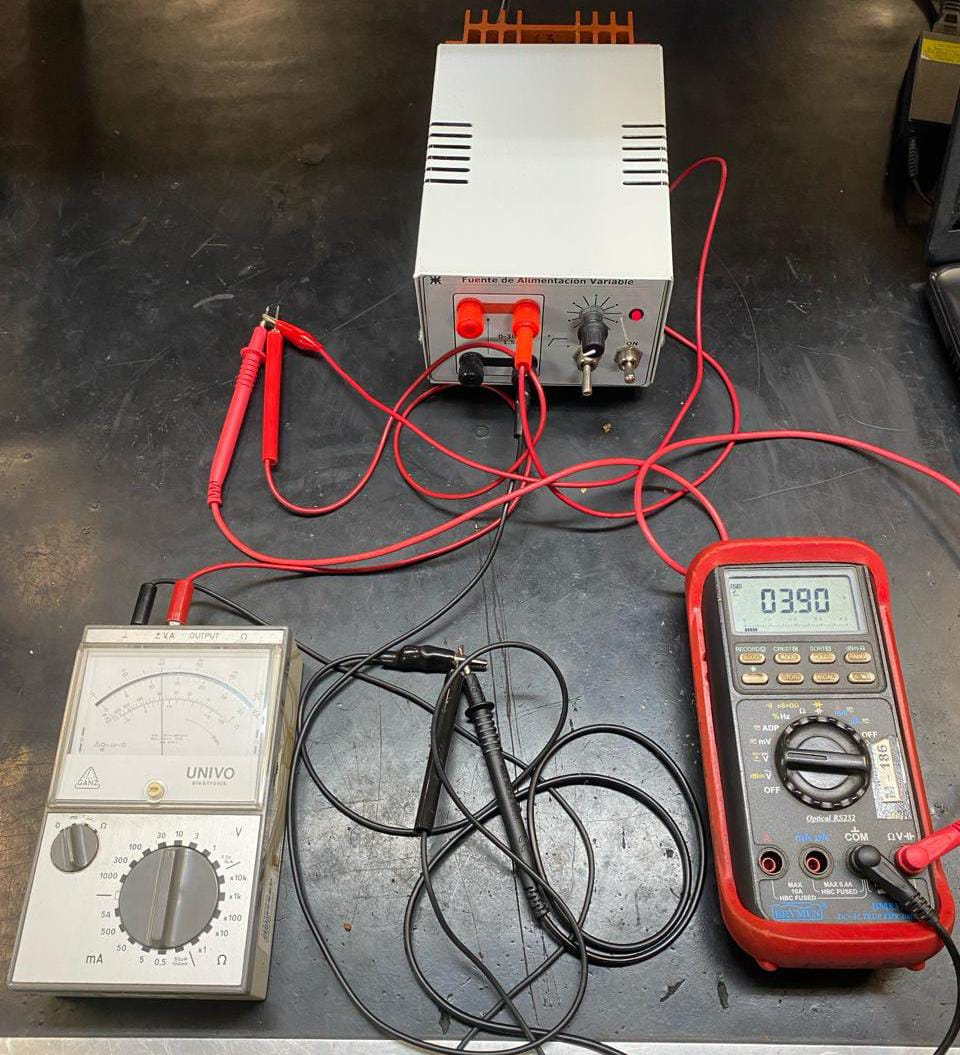
\includegraphics[width=0.35\textwidth]{Imagenes/Exp2.jpeg}
        \caption{Contrastación de un multímetro analógico con uno digital}
        \label{fig:contrast}
\end{figure}

\clearpage
 En base a los datos tabulados se confecciona la gráfica de corrección para representar cómo varia las mediciones con respecto al instrumento patrón. Sera útil para el usuario en caso de que quiera corregir de manera aproximadas el valor de su medición.

%FALTA lo de SUMAR y RESTAR en el grafico
%???

\begin{table}[H]
    \centering
    \scalebox{0.9}{
    \begin{tabular}{|c||c|c|c|c|}
    \hline
         & Instrumento constrastado & Patrón & Fecha & Operador \\
    \hline
        & Marca: Univo Elektronik & \makecell{Marca: UNI-T \\ Nro: UTC33C} & 26/03/2024 & Lucas Musso\\
    \hline
         &
        \multicolumn{4}{|c|}{
            %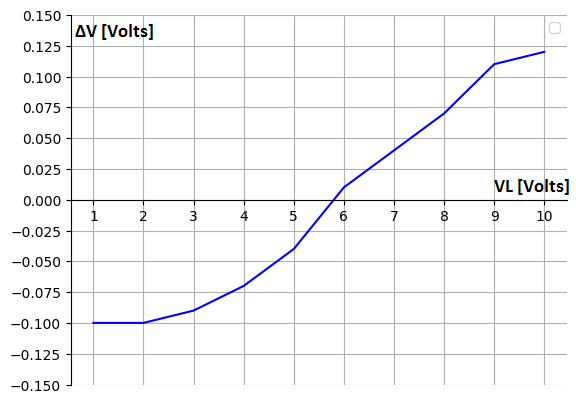
\includegraphics[width=\linewidth]{Imagenes/Grafica de correccion.png}
            \begin{tikzpicture}[scale=1]
    
    \def\scal{6/0.25}
    
    %datosLineaA
    \coordinate (a1) at (1,-0.07*\scal);
    \coordinate (a2) at (2,-0.12*\scal);
    \coordinate (a3) at (3,-0.14*\scal);
    \coordinate (a4) at (4,-0.13*\scal);
    \coordinate (a5) at (5,-0.15*\scal);
    \coordinate (a6) at (6,-0.14*\scal);
    \coordinate (a7) at (7,-0.14*\scal);
    \coordinate (a8) at (8,-0.14*\scal);
    \coordinate (a9) at (9,-0.14*\scal);
    \coordinate (a10) at (10,-0.23*\scal);

    
    %Ejex
    \draw[->] (0,0)--(11,0) node[right] {$VL_{(volts)}$};
    \foreach \x in {1,2,...,11}{
        \draw[line width=1pt,gray!40] (\x,-6)--(\x,6);
        \draw[shift={(\x,0)}] (0pt,2pt) -- (0pt,-2pt) node[below] {\footnotesize $\x$};
    }
    %Ejey
    \draw[<->] (0,-6)--(0,6) node[left]{$\Delta V_{(volts)}$};;
    \foreach \y in {-0.25,-0.20,-0.15,-0.10,-0.05,0.05,0.10,0.15,0.20}{
        \draw[line width=1pt,gray!40] (0,\y*6/0.25)--(11,\y*6/0.25);
        \draw[shift={(0,\y*6/0.25)}] (2pt,0pt) -- (-2pt,0pt) node [left] {\footnotesize $\y$} ;
    }
   \draw[shift={(0,0)}] (2pt,0pt) -- (-2pt,0pt) node [left] {\footnotesize $0$} ;
   \draw[line width=1pt,gray!40] (0,6)--(11,6);
   
    %Linea A
    \foreach \x  in {1,...,10}{
        \draw[line width=2pt,fill=black] (a\x) circle(2pt);
   }
   \foreach \x [evaluate={\y=int(\x+1);}] in {1,...,9}{
        \draw[line width=1pt,black] (a\x) -- (a\y);
   }
   \draw[line width=1pt,opacity=0.6,|-stealth] (10,-1)--(10,-4) node[midway,sloped,above]{$Sumar$};
   \draw[line width=1pt,opacity=0.6,|-stealth] (10,1)--(10,4) node[midway,sloped,below]{$Restar$};
   
\end{tikzpicture}


        } \\
        
         
    \hline
        \end{tabular}}
        \def\tablename{Tabla} 
        \caption{Mediciones del instrumento patrón y el máximo error absoluto}
        \label{tab:exp1b}
\end{table}


Se puede obtener la clase de exactitud del instrumento analógico a partir del máximo error absoluto medido (0.23 V para el experimento) a partir de la ecuación \ref{eq::clase}

\begin{equation}
    Clase= \frac{0.23 [V]}{10 [V]} \cdot 100\% = 2.3\%
\end{equation}

El "valor fiduciario" es también conocido como fondo de escala, y es el máximo valor medible en esa configuración del instrumento.

Por lo tanto, tiene coherencia con la clase especificada en la hoja de datos del instrumento, la cual es 2.5\%

Una vez calculada la clase del multímetro analógico, se procede a analizar cuan precisas son las mediciones del instrumento digital con respecto a las del instrumento de contraste. Para ello se realiza el cálculo de la relación de error::

\begin{equation}
    Relacion\;error = \frac{\Delta V_{MAX}}{error_{patron}} \ge 5
\end{equation}

Como ya se dijo antes, la relación de error debe ser mayor a 5 para toda la escala del instrumento patrón. Se puede representar la relación Medición - Error absoluto en una tabla para verificar hasta que esta condición se cumple (Tabla \ref{tab:relacionerror})

\begin{table}[h!]
    \centering
    \scalebox{0.99}{
    \begin{tabular}{|c||c|c|}
    \hline
         Medición & Error patrón & Relación error \\ \hline
        1   &  0.0108  &  21.30 \\ \hline
        2  &  0.0116  &  19.83 \\ \hline
        3  &  0.0124  &  18.55 \\ \hline
        4  &  0.0132  &  17.42 \\ \hline
        5  &  0.0140  &  16.43 \\ \hline
        6  &  0.0148  &  15.54 \\ \hline
        7  &  0.0156  &  14.74 \\ \hline
        8  &  0.0164  &  14.02 \\ \hline
        9  &  0.0172  &  13.37 \\ \hline
        10 &  0.0180  &  12.78 \\ \hline
        \end{tabular}}
        \def\tablename{Tabla} 
        \caption{Relaciones de errores entre instrumento patrón y de contraste}
        \label{tab:relacionerror}
\end{table}

\begin{figure}[H]
    \centering
    \begin{tikzpicture}[scale=1]
\def\scal{6/10}
\def\des{12}
    
    %datosLineaA
    \coordinate (a1) at (1,21.3*\scal-\des*\scal);
    \coordinate (a2) at (2,19.83*\scal-\des*\scal);
    \coordinate (a3) at (3,18.55*\scal-\des*\scal);
    \coordinate (a4) at (4,17.42*\scal-\des*\scal);
    \coordinate (a5) at (5,16.43*\scal-\des*\scal);
    \coordinate (a6) at (6,15.54*\scal-\des*\scal);
    \coordinate (a7) at (7,14.74*\scal-\des*\scal);
    \coordinate (a8) at (8,14.02*\scal-\des*\scal);
    \coordinate (a9) at (9,13.37*\scal-\des*\scal);
    \coordinate (a10) at (10,12.78*\scal-\des*\scal);

    %Ejex
    \draw[->] (0,0)--(11,0) node[midway,below={5mm}] {Medición};
    \foreach \x in {0,1,2,...,11}{
        \draw[line width=1pt,gray!40] (\x,0) -- (\x,6);
        \draw[shift={(\x,0)}] (0pt,2pt) -- (0pt,-2pt) node[below] {\footnotesize $\x$};
    }
    %Linea A
    \foreach \c in {1,...,10}{
        \draw[line width=1pt,gray!40] let \p1 = (a\c)in (11,\y1)--(0,\y1);
        \draw[] let \p1= (a\c)in (2pt,\y1) -- (-2pt,\y1);
   }
    \foreach \x  in {1,...,10}{
        \draw[line width=2pt,fill=black] (a\x) circle(1pt);
   }
   \foreach \x [evaluate={\y=int(\x+1);}] in {1,...,9}{
        \draw[line width=1pt,black] (a\x) -- (a\y);
   }

   
    %Ejey
    \draw[->] (0,0)--(0,6) node[midway,sloped,above={15mm}]{Relación error};
    \foreach \c in {1,2,4,6,10}{
        
    }
    
   \draw[] let \p1= (a1)in (2pt,\y1) -- (-2pt,\y1) node[left] {\footnotesize $21.30$};
   \draw[] let \p1= (a2)in (2pt,\y1) -- (-2pt,\y1) node[left] {\footnotesize $19.83$};
   \draw[] let \p1= (a3)in (2pt,\y1) -- (-2pt,\y1) node[left] {\footnotesize $18.55$};
   \draw[] let \p1= (a4)in (2pt,\y1) -- (-2pt,\y1) node[left] {\footnotesize $17.42$};
   \draw[] let \p1= (a5)in (2pt,\y1) -- (-2pt,\y1) node[left] {\footnotesize $16.43$};
   \draw[] let \p1= (a6)in (2pt,\y1) -- (-2pt,\y1) node[left] {\footnotesize $15.54$};
   \draw[] let \p1= (a7)in (2pt,\y1) -- (-2pt,\y1) node[left] {\footnotesize $14.74$};
   \draw[] let \p1= (a8)in (2pt,\y1) -- (-2pt,\y1) node[left] {\footnotesize $14.02$};
   \draw[] let \p1= (a9)in (2pt,\y1) -- (-2pt,\y1) node[left] {\footnotesize $13.37$};
   \draw[] let \p1= (a10)in (2pt,\y1) -- (-2pt,\y1) node[left] {\footnotesize $12.78$};

 
\end{tikzpicture}
    \caption{Relaciones de errores entre instrumento patrón y de contraste}
    \label{fig:relacionerror}
\end{figure}






\newpage
\subsection{Experimento 2}

%Habria que poner la foto del experimento reaaaaal


Para el segundo experimento de este práctico, se plantea realizar una medición indirecta de la resistencia de una probeta (cable). Para esto se establecerá una corriente fija a través de esta y luego se medirá la tensión a los bornes de la probeta para así emplear la Ley de Ohm y obtener el valor de la resistencia.

En la figura \ref{fig:CircExp2}, se puede apreciar el circuito teórico propuesto para este experimento. 

\begin{figure}[H]
    \centering
    \begin{circuitikz} [scale=1,american, transform shape]
\def\scal{1};
\draw (0,-2) to[I] (0,2)  (4.5,2) edge[dashed] (7.5,2) (0,2) to[short,-o] (4.5,2) ;
\draw (7.5,2) to[short,o-] (8,2)to[R, l=$R_{probe}$] (8,-2) (7.5,-2) edge[dashed](4.5,-2) (4,-2) to[short,-o](4.5,-2) (8,-2) to[short,-o](7.5,-2);
\draw (4,2) to[rmeterwa, t=V, v=$v$, o-o] (4,-2);
\draw (4,-2) to[rmeterwa, t=I, i=$i$, o-] (0,-2);

\end{circuitikz}{}
    \caption{Circuito experimento 2}
    \label{fig:CircExp2}
\end{figure}

Además de esta medición, se realizarán los cálculos necesarios para determinar la incertidumbre en esa medición.

En este ensayo, se emplearon algunos instrumentos provistos por el laboratorio, entre ellos: una fuente de corriente con una tensión de alimentación de 12 V y la probeta, que consistía en un tramo de cable enrollado de 20 m $\pm$ 20cm de largo, con un arrollamiento no inductivo (para disminuir al máximo los posibles efectos auto inductivos del cable). Además de esto, se utilizaron dos multímetros de la marca UNI-T. El primer multimetro utilizado era un modelo UT890C, utilizado como miliamperímetro y el segundo fue un modelo UT33C, empleado como voltímetro. 

Antes de realizar el experimento se decidió medir la resistencia de la probeta de manera directa, con el multímetro configurado para comprobar continuidad. Este indicaba que efectivamente había continuidad y que el cable tenía una resistencia de $1.5 \Omega$. 

\subsubsection{Mediciones}

Se conecto la fuente de alimentación, de 12 V, al circuito de la fuente de corriente. Luego se conectaron los bornes de salida de esta, uno a la probeta y el otro al multímetro que mediría la corriente que circula por la probeta. Por supuesto, el otro extremo de la probeta y la otra punta del multímetro fueron conectadas entre sí (figura \ref{fig:foto2}).

\begin{figure}[h!]
    \centering    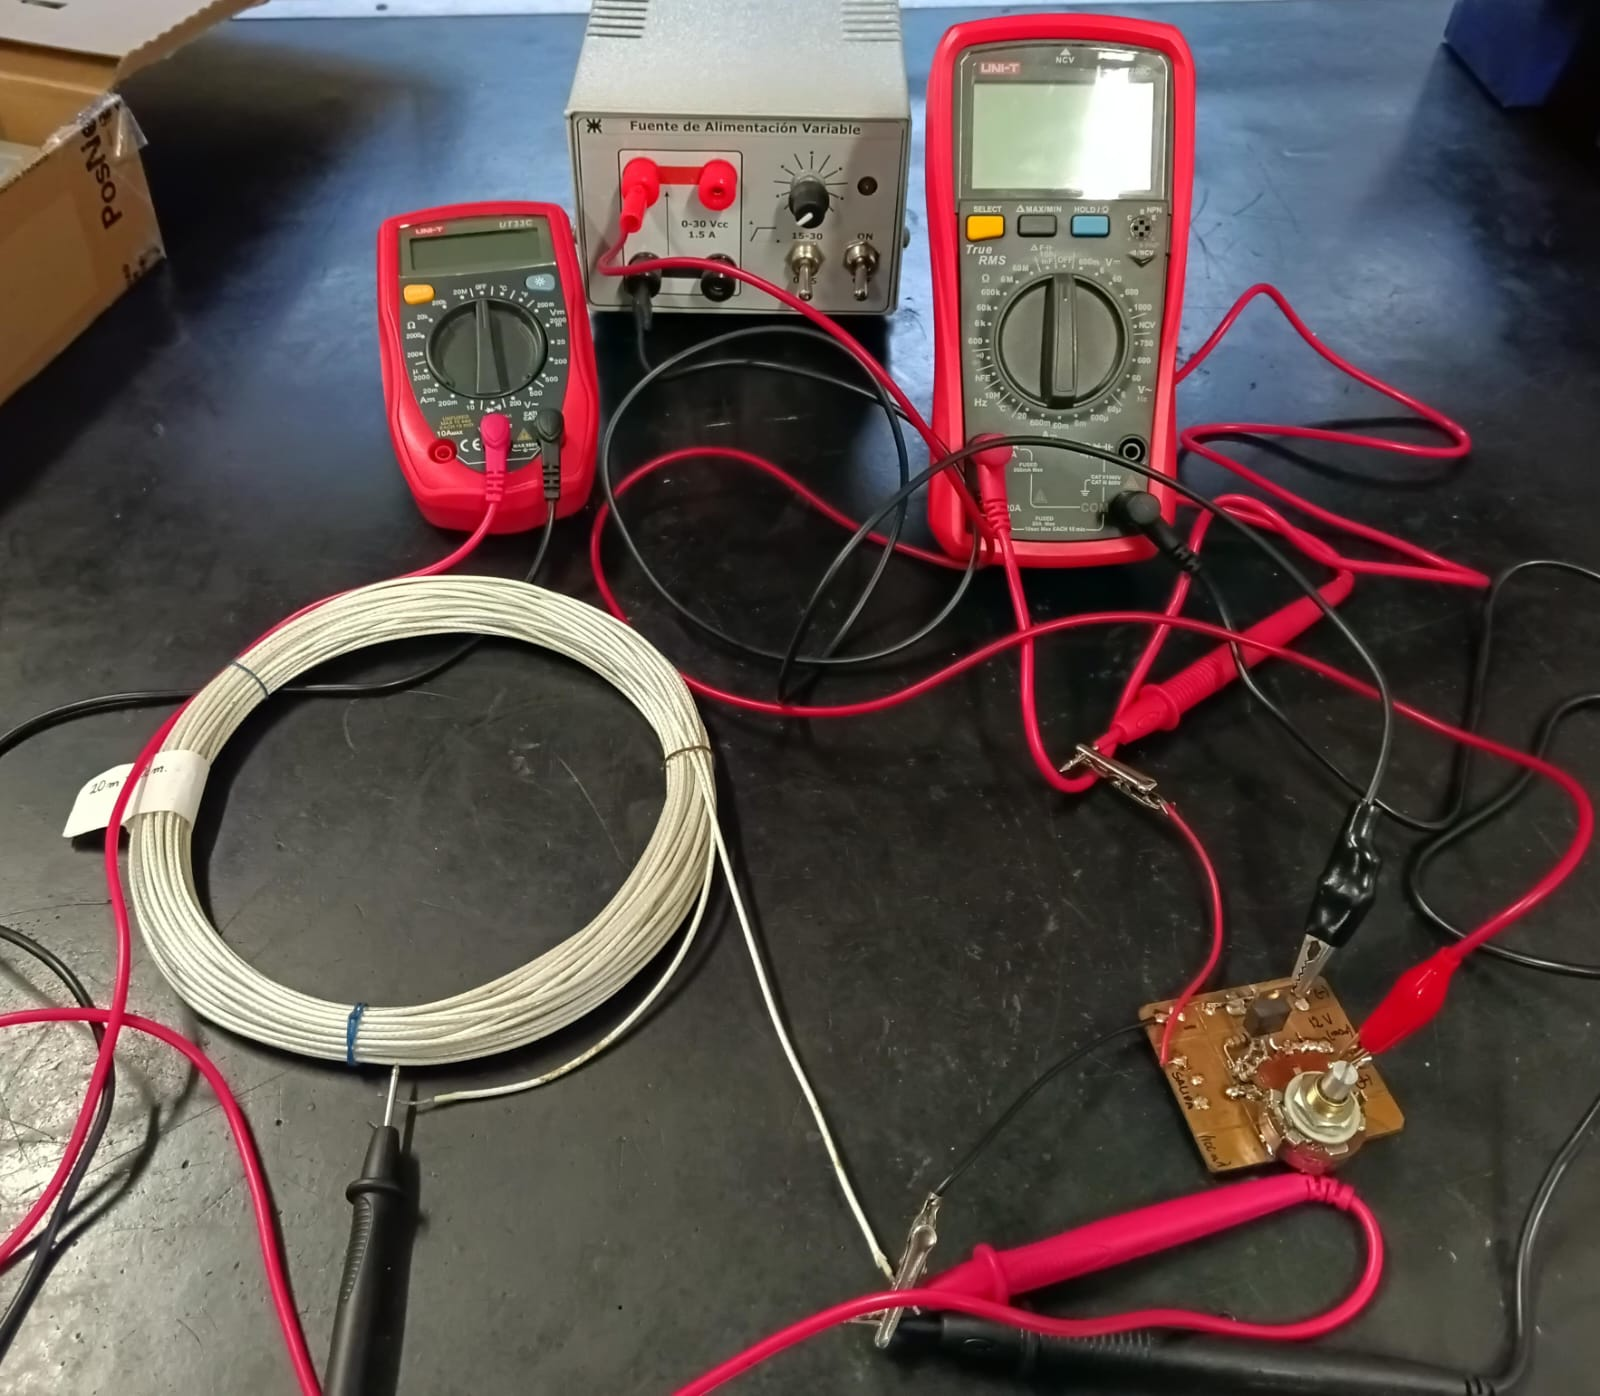
\includegraphics[width=0.5\textwidth]{Imagenes/WhatsApp Image 2024-04-11 at 18.13.00.jpeg}
    \caption{Circuito experimento 2}
    \label{fig:foto2}
\end{figure}

Se estableció una corriente de 100 mA a través de la probeta y se procedió a medir la diferencia de potencial que había entre sus bornes. A partir de este valor se calculó la resistencia del cable cómo se ve a continuación en la tabla \ref{tab:exp2a}.


\begin{table}[h!]
    \centering
    \begin{tabular}{|c|c|}
    \hline
        V & 101 $mV$ \\
    \hline
        I & 100 $mA$ \\
    \hline
        R = V/I & 1.01 $\Omega$ \\ 
    \hline
        \end{tabular}
        \def\tablename{Tabla} 
        \caption{Mediciones sobre la probeta}
        \label{tab:exp2a}
\end{table}

Se obtuvo como resultado un valor de 1.01 $\Omega$, sin embrago, aún queda analizar el nivel de incertidumbre que contiene esta medición. 

\subsubsection{Cálculo de Incertidumbre}

Al realizar una medición indirecta se debe tener en cuenta que la incertidumbre del valor calculado, se verá afectada por los errores de las mediciones implicadas. Por lo tanto, para el cálculo de la incertidumbre en la medición de la resistencia, habrá que tener en cuenta la incertidumbre en las mediciones de corriente y tensión.

El valor de la resistencia resulta ser el cociente entre la tensión y la corriente, por ende, el error relativo máximo total es la suma de los errores relativos máximos parciales, es decir:

\begin{equation}
    \frac{\Delta R}{R} = \frac{\Delta V}{V} + \frac{\Delta I}{I}
    \label{sumaErr}
\end{equation}

Los errores máximos relativos se calculan a partir de las mediciones efectuadas, teniendo en cuenta las especificaciones del multímetro utilizado. 

Antes de calcular el error máximo relativo, debemos averiguar el error de cada medición. Para esto se utilizan los datos que cada fabricante indica en el manual del instrumento. 

La medición de corriente fue efectuada con el miliamperímetro del tester UT890C en el rango de 600 mA. Las especificaciones para el cálculo de la incertidumbre ($\Delta I$) de este las podemos encontrar en el Anexo \ref{sec:Información Instrumentos} en la tabla \ref{tab:DCI_UT890C}. En base a esto, el cálculo quedaría así:

\begin{equation}
    \Delta I = \pm \left( \cfrac{1.2 \cdot 100 [mA]}{100} + 0.5 [mA] \right) = \pm 1.7 [mA]  
\end{equation}

En el caso de la tensión, que fue medida con el voltímetro del tester UT33C en el rango de 200 mV y cuyas especificaciones se pueden ver en la tabla \ref{tab:DCV_UT33C} del Anexo \ref{sec:Información Instrumentos}, la incertidumbre resultó ser:

\begin{equation}
    \Delta V = \pm \left( \cfrac{0.5 \cdot 101 [mV]}{100} + 0.2 [mV] \right) = \pm 0.705 [mV]  
\end{equation}

Con los valores recién obtenidos y mediante lo calculado siguiendo la ecuación \ref{sumaErr}, se confeccionó la tabla \ref{tab:exp2b}, presentada a continuación.

\begin{table}[h!]
    \centering
    \scalebox{1}{
    \begin{tabular}{|c||c|c|c|c|}
    \hline
         ---- & $x$ & $\Delta x$ & $\cfrac{\Delta x}{x}$ & $\cfrac{\Delta x}{x} \cdot 100$ \\
    \hline
        V & 101 $mV$ & 0.705 $mV$ & $6.98 \cdot 10^{-3}$ & $0.698 \%$ \\
    \hline 
        I & 100 $mA$ & 1.7 $mA$ & 0.017 & $1.7 \%$ \\
    \hline
        R = V/I & 1.01 $\Omega$ & $24.2 \cdot 10^{-3}$ $\Omega$ & $23.98 \cdot 10^{-3}$ & 2.398\% \\
         
    \hline
        \end{tabular}}
        \def\tablename{Tabla} 
        \caption{Incertidumbre y error relativo de las mediciones sobre la probeta}
        \label{tab:exp2b}
\end{table}

La incertidumbre de la resistencia ($\Delta R$) fue obtenida luego de emplear la ecuación \ref{sumaErr} y multiplicar el resultado por el valor de resistencia calculada. 

\begin{equation*}
    \frac{\Delta R}{R} = \frac{\Delta V}{V} + \frac{\Delta I}{I}
    \hspace{0.5cm}
    \Longrightarrow
    \hspace{0.5cm}
    \frac{\Delta R}{R} = 6.98 \cdot 10^{-3} + 0.017 = 23.98 \cdot 10^{-3}
\end{equation*}

\begin{equation*}
    \Delta R = 23.98 \cdot 10^{-3} \cdot 1.01 [\Omega] = 24.2 \cdot 10^{-3} [\Omega]
\end{equation*}

Entonces, como resultado final teniendo en cuenta la incertidumbre queda:

\begin{equation*}
    R_{probe} = 1.01 \pm 0.0242 [\Omega]
\end{equation*}

En base a estos resultados, se puede decir que la medición de la resistencia por este método tiene una precisión bastante buena, teniendo un error de solamente unos cuantos miliohm, a diferencia de la escala más baja del multímetro con el que la medimos al principio, que tiene una incertidumbre de al menos 0.5 $\Omega$ (fijos), más el error porcentual del 0.8$\%$ sobre la medición (ver tabla \ref{tab:DCR_UT33C}, del Anexo \ref{sec:Información Instrumentos}).

\newpage
\subsection{Experimento 3}

Como objetivo del experimento 3, se planteó realizar la medición de la resistencia de un sistema de puesta a tierra, mediante el método visto en el experimento anterior. 

\subsubsection{Medición en el laboratorio}

Para este ensayo, se empleará un Telurímetro, presentado en la sección de \textit{\nameref{sec:MTmrspt}}, del Marco Teórico; de la marca UNI-T, modelo UT522. Este es un telurímetro de 3 puntas, donde una corresponde al electrodo de corriente, otra al de tensión y la tercera punta se conecta a la toma a tierra. En esta última punta están conectadas internamente la otra terminal del multímetro y amperímetro correspondientes a los demás electrodos (se sigue teniendo 4 puntos como en la sección anterior, pero solo se ven 3 porque dos están conectados internamente). 

El ensayo se realizó el día 4 de abril del año 2024, en el laboratorio central de electrónica de la Universidad Tecnológica Nacional, Facultad Regional Córdoba. Para este, se implementó el siguiente circuito (figura \ref{fig:circtel}), con el telurímetro antes presentado.

\begin{figure}[h!]
        \centering        
        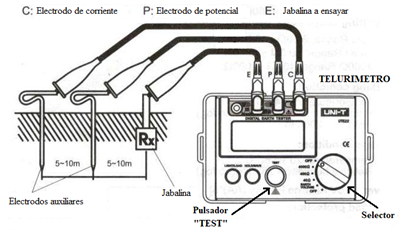
\includegraphics[width=0.8\textwidth]{Imagenes/Telurimetro.png}
        \caption{Esquema de conexión del Telurímetro UT522}
        \label{fig:circtel}
\end{figure}

Como se explico en el Marco Teórico y se puede ver en la figura \ref{fig:circtel}, para la medición de la resistencia de un sistema de puesta a tierra específico ($R_x$) se deberían insertar en el terreno los electrodos auxiliares, pero debido a que se realizó en el laboratorio, el cual cuenta con un piso de baldosas (haciendo imposible o poco práctica la inserción de los electrodos), se utilizaron dos electrodos auxiliares consistentes en dos planchas de acero de 20cm x 20cm (figura \ref{fig:electrodos}), que se apoyaran sobre el piso cubierto con un paño (trapo de piso) humedecido con bastante agua. 

\begin{figure}[h!]
        \begin{subfigure}[b]{0.5\textwidth}
        \centering  
        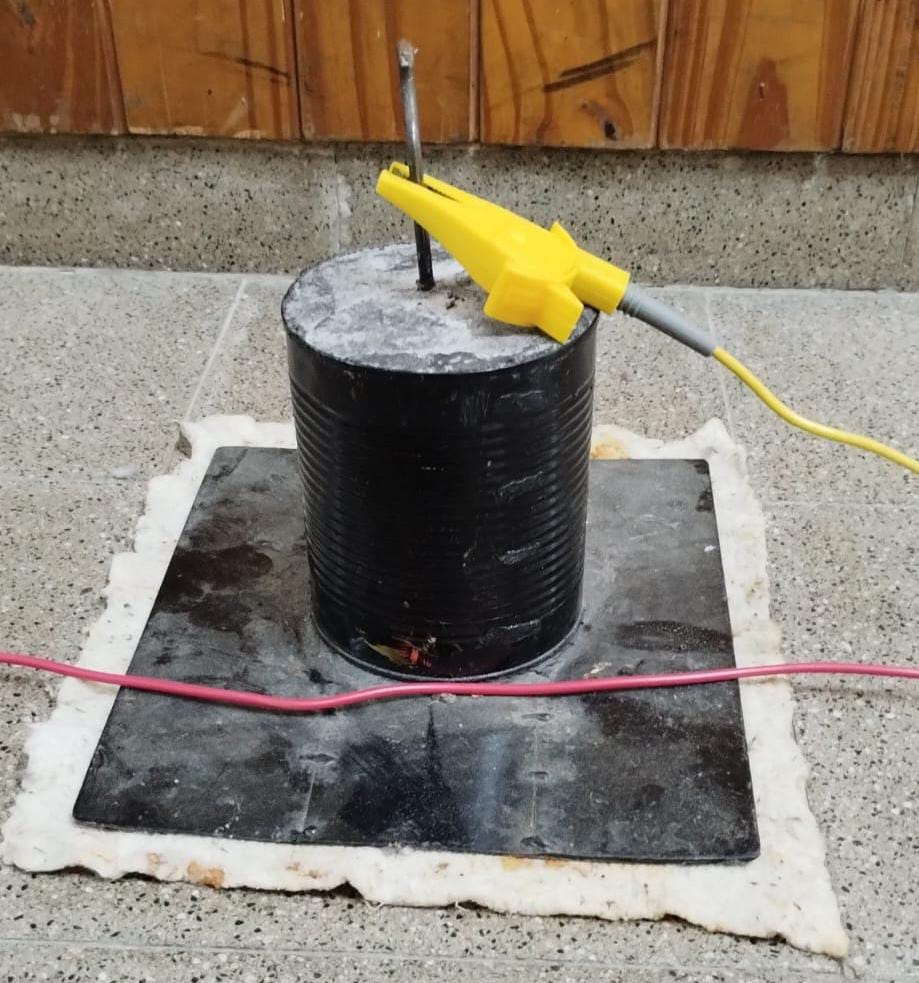
\includegraphics[width=0.6\textwidth]{Imagenes/ElectrodoTel.jpeg}
        \caption{Electrodos auxiliares utilizados}
        \label{fig:electrodos}
    \end{subfigure}
    \hfill
    \begin{subfigure}[b]{0.49\textwidth}
        \centering
        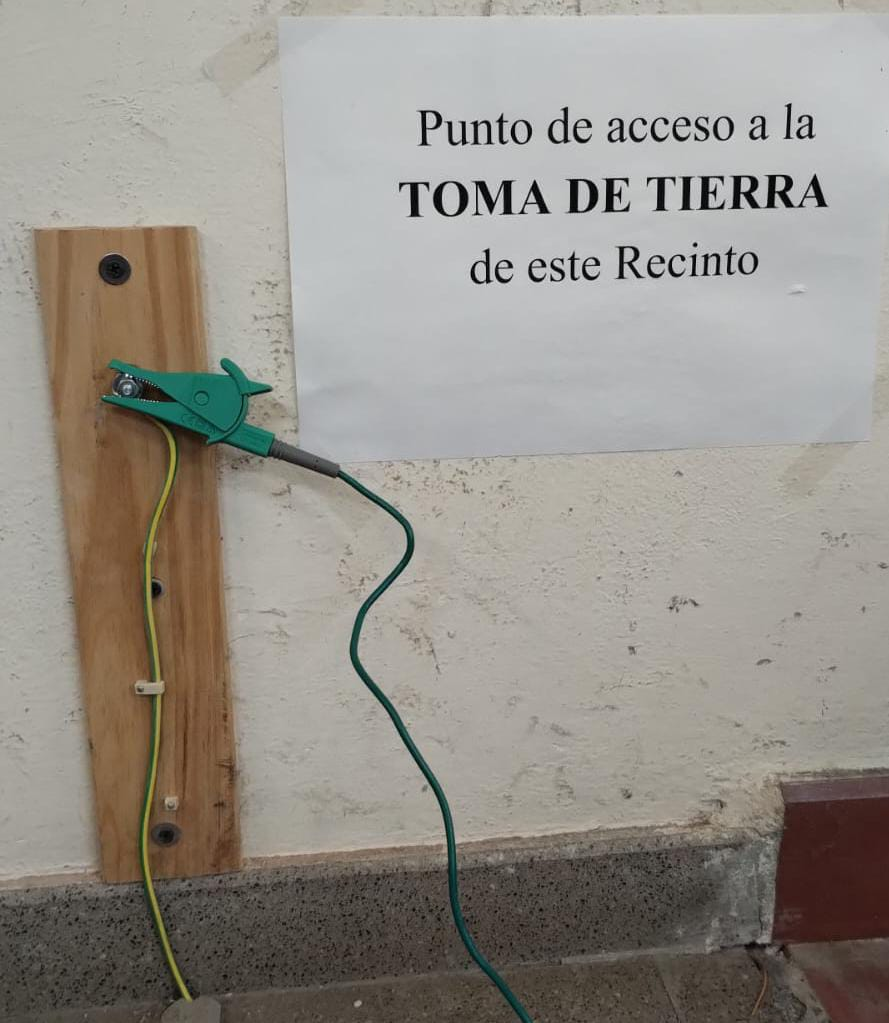
\includegraphics[width=0.57\textwidth]{Imagenes/TomaTierra.jpeg}
        \caption{Toma a tierra del laboratorio central}
        \label{fig:tomatierra}
    \end{subfigure}
    \caption{Puntos de conexión de los cables del telurímetro}
\end{figure}

Los electrodos se dispusieron en el pasillo externo, a 10 m entre sí y a aproximadamente 10 m de la toma a tierra del laboratorio central (figura \ref{fig:tomatierra}). Cabe destacar, que los electrodos fueron colocados en el pasillo, ya que en realidad la puesta a tierra del laboratorio consiste en una malla conductora colocada debajo de todo el solado del recinto. 

Una vez colocados los electrodos y conectados estos al telurímetro, se comenzó con las mediciones, comenzando desde el rango más alto del instrumento hasta llegar a la medición más precisa de acuerdo con el valor a medir. 

Siguiendo este método, el telurímetro mostró un un valor de resistencia de la jabalina de:

\begin{figure}[h!]
    \begin{minipage}{0.6\textwidth}\
        \centering  
        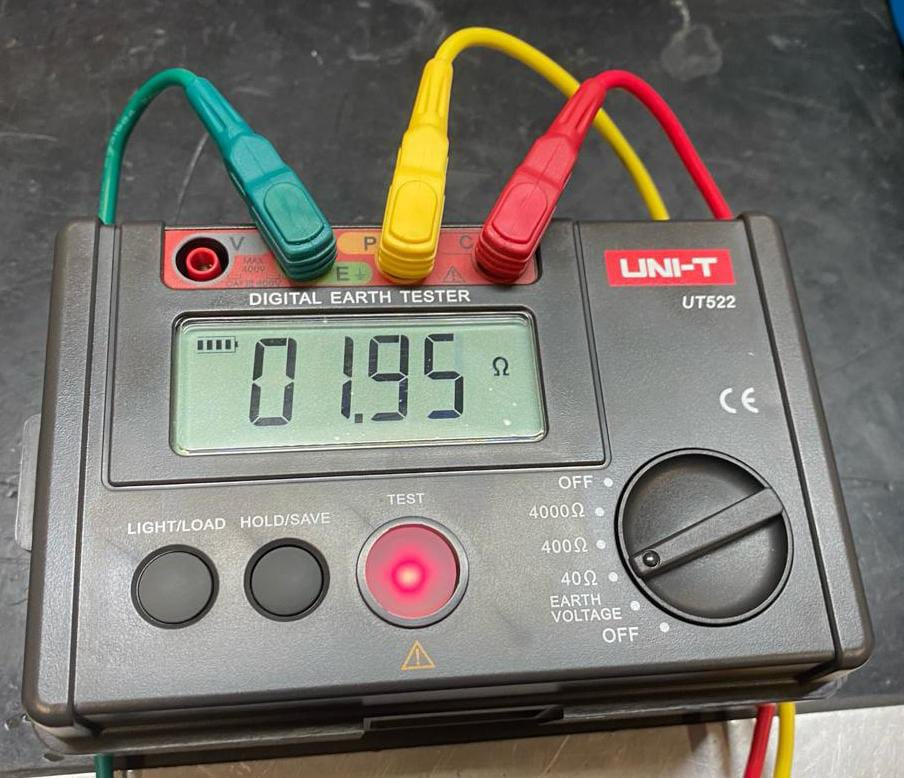
\includegraphics[width=0.6\textwidth]{Imagenes/Lecttel.jpeg}
        \caption{Lectura en el telurímetro}
        \label{fig:lecttel}
    \end{minipage}
    \begin{minipage}{0.39\textwidth}\
        \begin{equation*}
            R_{Jabalina} = 1.95 [\Omega]
        \end{equation*}
    \end{minipage}
\end{figure}

Una vez obtenido este valor, se procedió a calcular la incertidumbre de esta medición. Para esto se tuvieron en cuenta los datos de precisión del instrumento, consignados en la tabla \ref{tab:Telurimetro}, del Anexo \ref{sec:Información Instrumentos}; y la fórmula antes presentada para el cálculo de incertidumbre.

\begin{equation}
    \Delta R = \pm \left( \cfrac{2.0 \cdot 1.95 [\Omega]}{100} + 20 \cdot 10 [m\Omega] \right) = \pm 0.239 [\Omega]  
\end{equation}

Quedando como resultado de la medición el siguiente valor de resistencia:

\begin{equation*}
    R_{Jabalina} = 1.95 \pm 0.239 [\Omega]
\end{equation*}

Se puede ver que el sistema de puesta a tierra de nuestra facultad, está dentro de la norma establecida por la ley, que exige que la resistencia de este tipo de sistemas, no puede superar los 5$\Omega$. Según lo indicado por el telurímetro y suponiendo la mayor incertidumbre, el valor de resistencia no supera los 2.5$\Omega$.

Luego de realizada esta medición se reemplazó el instrumento por otro telurímetro, uno modelo MI-2124 de la marca METREL. Este segundo telurímetro era de cuatro puntos por lo que tenía cuatro entradas en lugar de tres como el anterior, y la conexión interna entre voltímetro y amperímetro no estaba. Sin embargo, esa misma conexión se realizo externamente, los cables correspondientes a un terminal del voltímetro y uno del amperímetro, se conectaron ambos a la toma a tierra del laboratorio y los dos restantes, a los electrodos.

Una vez instalado el dispositivo y los electrodos, se procedió a realizar la medición (figura \ref{fig:tel2lab}). 

\begin{figure}[h!]
        \centering        
        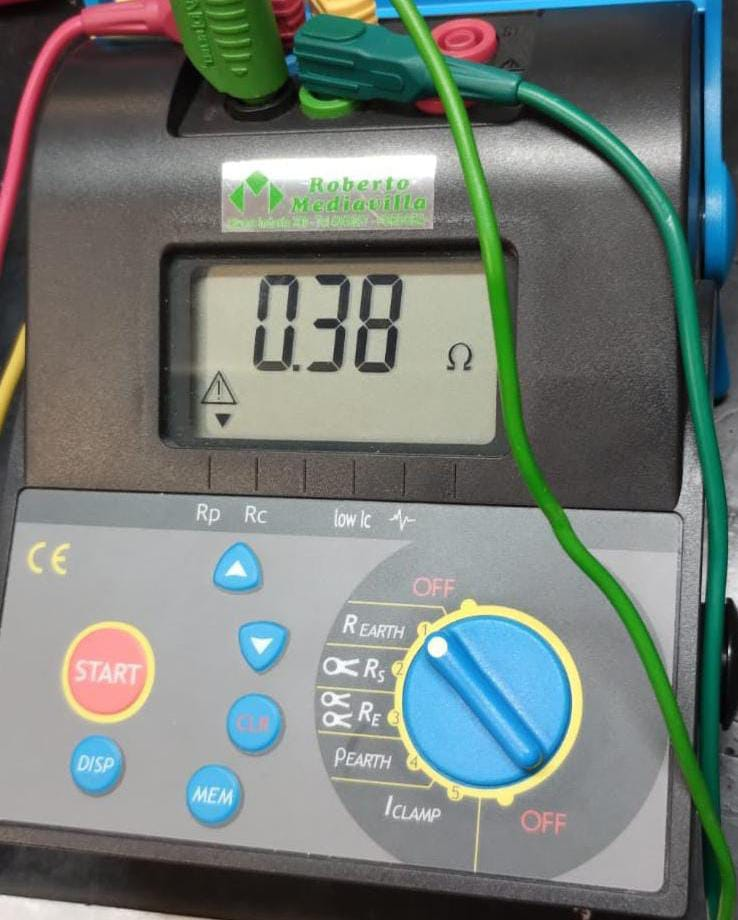
\includegraphics[width=0.3\textwidth]{Imagenes/tel2lab.jpeg}
        \caption{Medición con Telurímetro MI-2124}
        \label{fig:tel2lab}
\end{figure}

En este caso, no hizo falta el procedimiento de ir bajando de escala, ya que era de auto-rango, sin embargo se puede ver que la resistencia medida es mucho menor (0.38$\Omega$). 

En cuanto a la incertidumbre en la medición, aplicamos el cálculo anterior, con las especificaciones del nuevo telurímetro (Anexo \ref{sec:Información Instrumentos}, tabla \ref{tab:TelurMI2124}). 

\begin{equation*}
    \Delta R = \pm \left( \cfrac{2 \cdot 0.38 [\Omega]}{100} + 3 \cdot 10 [m\Omega] \right) = \pm 0.0376 [\Omega]  
\end{equation*}

Según esta segunda medicion tenemos que la resistencia del sistema de puesta a tierra es de:

\begin{equation*}
    R_{Jabalina} = 0.38 \pm 0.0376 [\Omega]
\end{equation*}

La diferencia entre las lecturas (incluyendo su incertidumbre) no debería ser tan grande, se supone que se debían obtener lecturas similares. Se cree que esta diferencia puede deberse a la utilización de electrodos distintos a los que vienen con el dispositivo y que estos agregaron cierta resistencia de contacto adicional debido a una mala conexión, que puede haberse corregido para la segunda medición. Afortunadamente, ambas mediciones indicaban que el sistema del laboratorio estaba dentro de la norma, por lo que aunque exista esta diferencia, no se debería presentar ningún problema durante su utilización.

\subsubsection{Medición en el patio frontal}

Adicionalmente, se realizó otro ensayo de la resistencia del sistema de puesta a tierra en el patio frontal de la facultad, donde esta vez si se emplearon las estacas que vienen con el dispositivo. La toma a tierra utilizada en esta ocasión se encontraba dentro de otro laboratorio que daba al patio.



Luego de colocar las estacas, se midió la resistencia de la puesta a tierra en ese punto y el telurímetro UNI-T reveló un valor más bajo que en la medición anterior (figura \ref{fig:tel1patio}). 

En este caso, el valor era de 0.27$\Omega$, que junto con la incertidumbre queda:

\begin{equation*}
    \Delta R = \pm \left( \cfrac{2.0 \cdot 0.27 [\Omega]}{100} + 20 \cdot 10 [m\Omega] \right) = \pm 0.2054 [\Omega]    
\end{equation*}

\begin{equation*}
    R_{Jabalina_1} = 0.27 \pm 0.2054 [\Omega]
\end{equation*}

En esta medición podemos ver que la exactitud de este multímetro quizá no es la más adecuada para medir una resistencia tan pequeña, ya que la incertidumbre es muy similar al valor medido. En otras palabras el error máximo que puede haber en la medición es de aproximadamente el 100$\%$ del valor. 

Manteniendo exactamente la misma disposición e incluso los mismos cables se cambió el telurímetro por el de la marca METREL, y el resultado fue el de la figura \ref{fig:tel2patio}.

\begin{figure}[h!]
        \begin{subfigure}[b]{0.5\textwidth}
        \centering  
        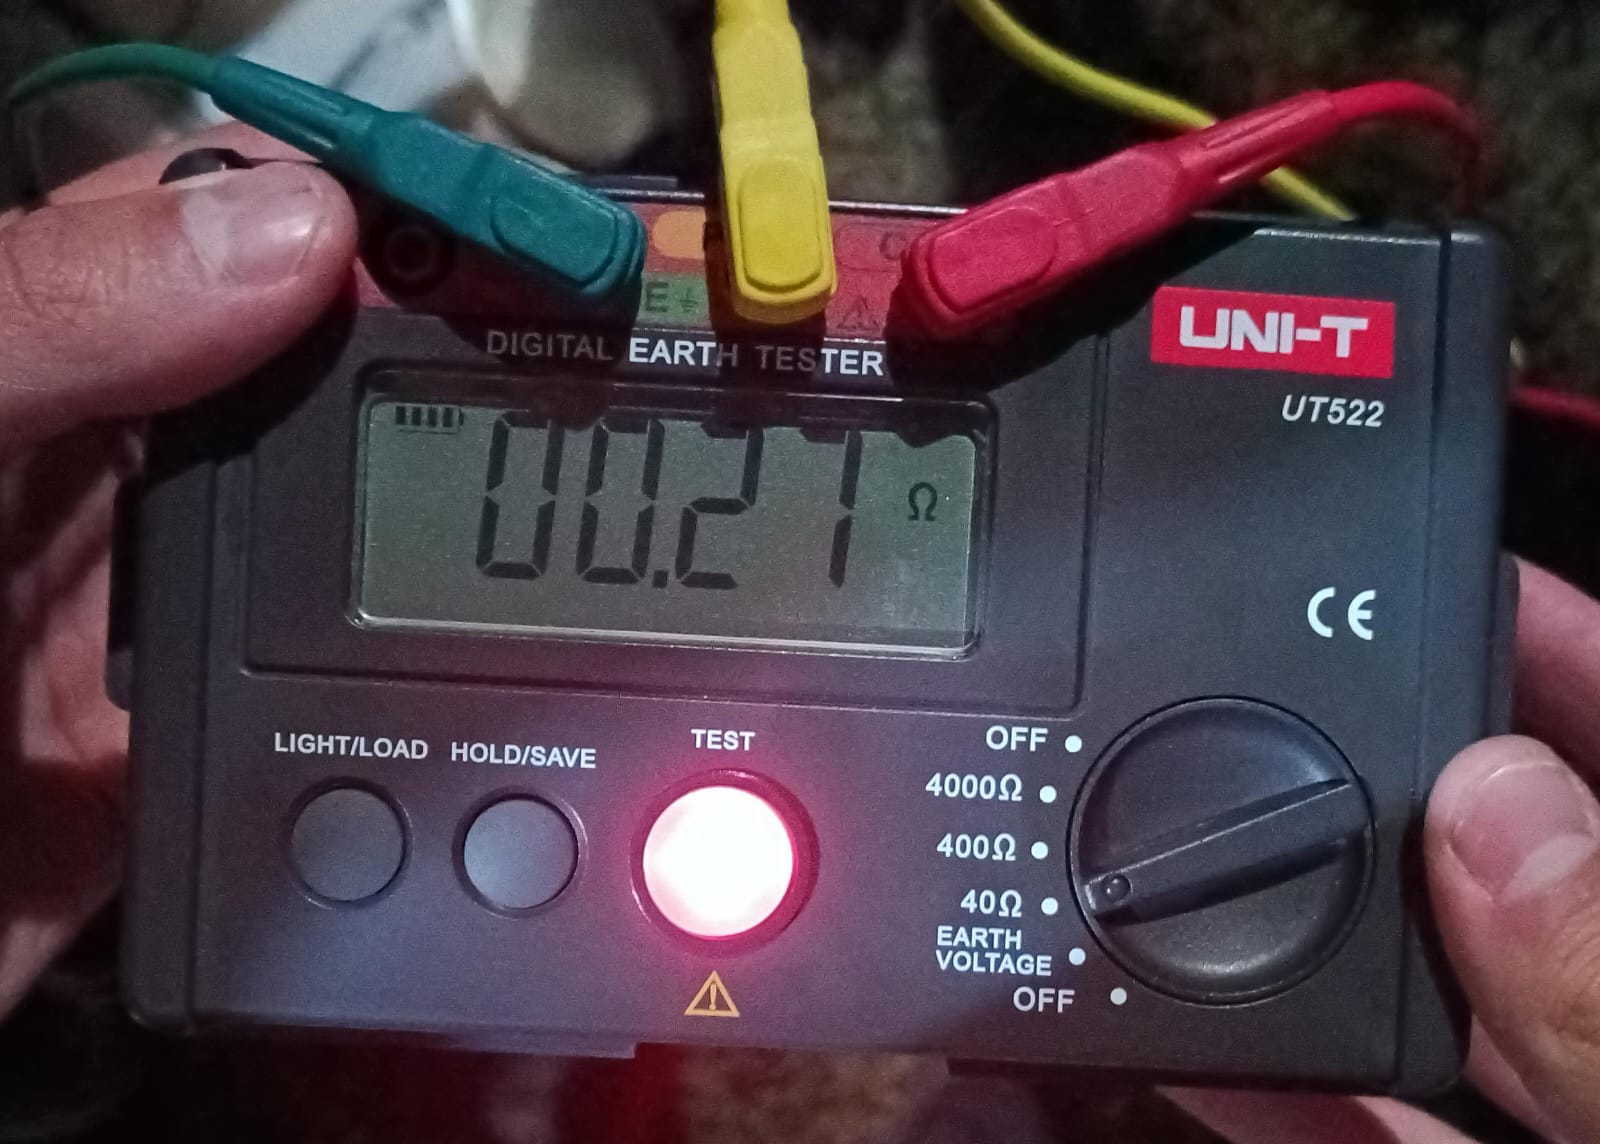
\includegraphics[width=0.8\textwidth]{Imagenes/tel1patio.jpeg}
        \caption{Medición con Telurímetro UT-522}
        \label{fig:tel1patio}
    \end{subfigure}
    \hfill
    \begin{subfigure}[b]{0.49\textwidth}
        \centering
        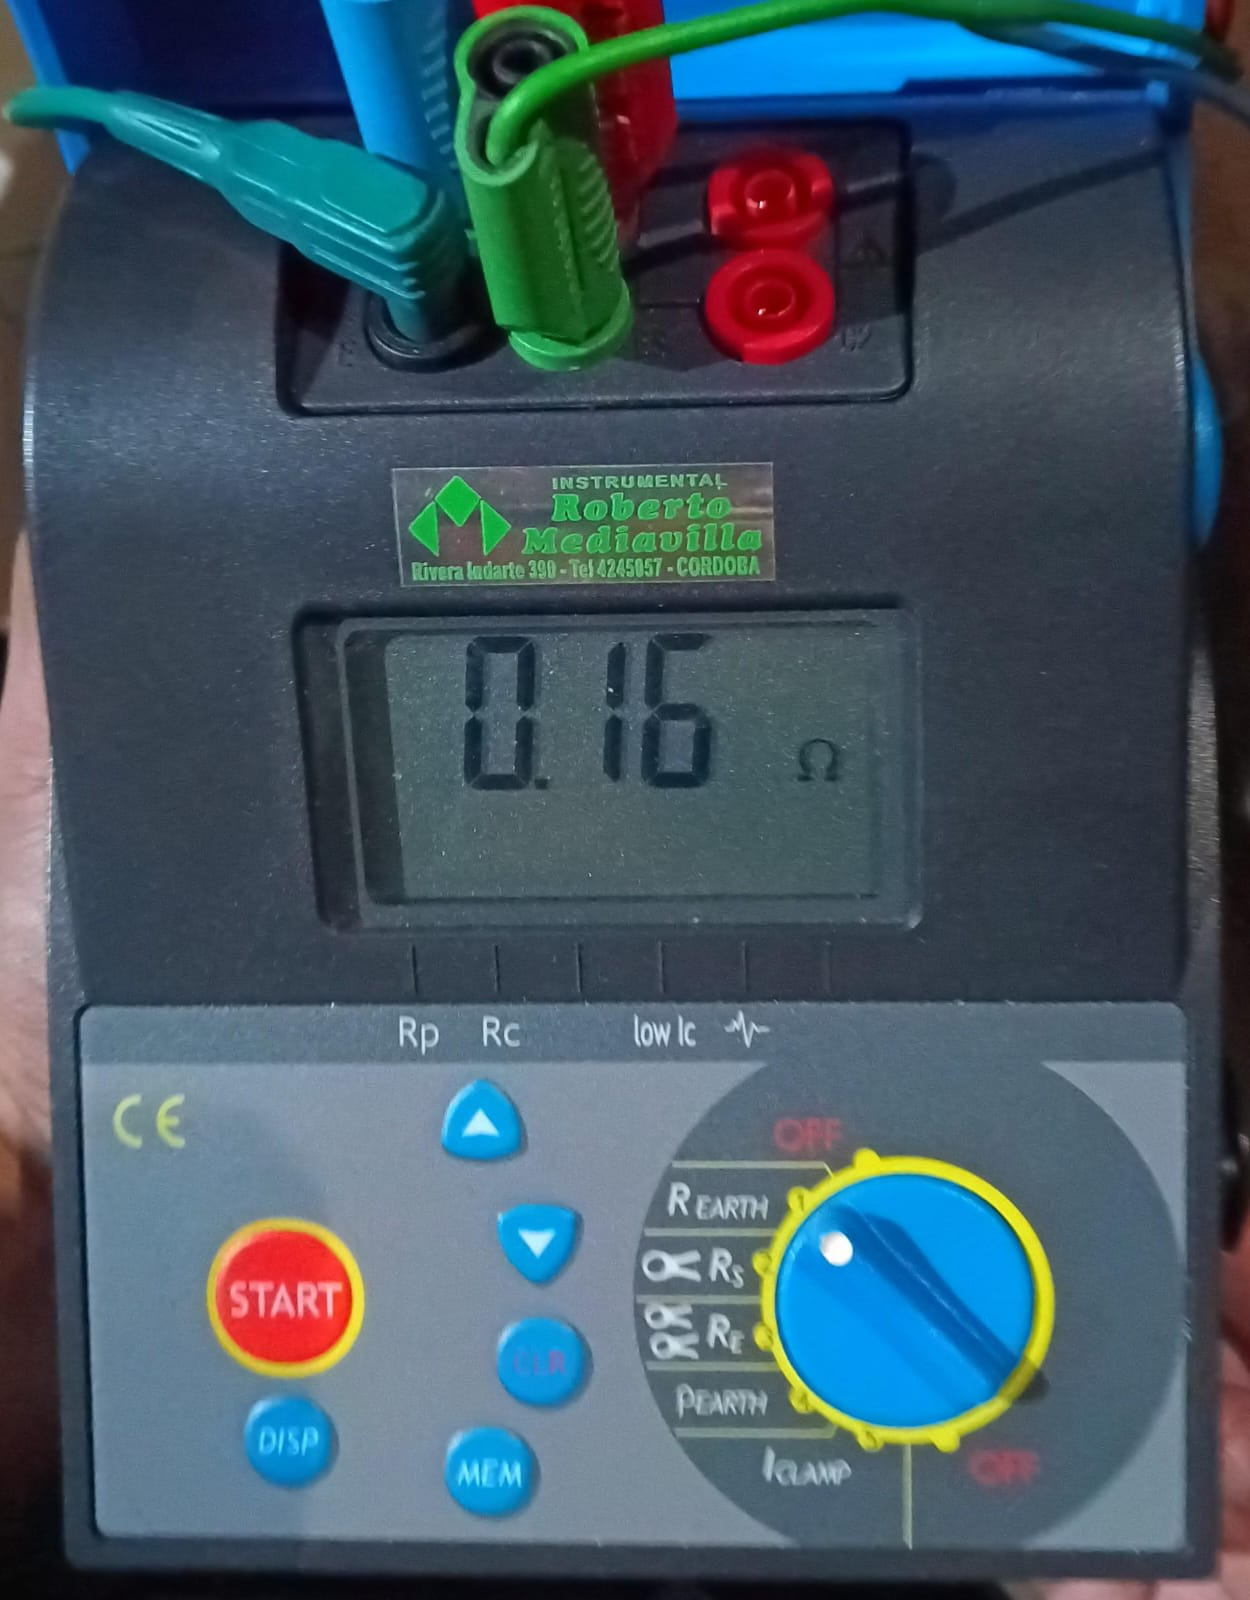
\includegraphics[width=0.45\textwidth]{Imagenes/tel2patio.jpeg}
        \caption{Medición con Telurímetro MI-2124}
        \label{fig:tel2patio}
    \end{subfigure}
    \caption{Mediciones del sistema de puesta a tierra en el patio}
\end{figure}

A simple vista se aprecia que la diferencia entre mediciones es mucho menor, pero este telurímetro sigue mostrando un valor de resistencia menor que el de marca UNI-T.

Calculamos la incertidumbre de este última medición y obtenemos:

\begin{equation*}
    \Delta R = \pm \left( \cfrac{2 \cdot 0.16 [\Omega]}{100} + 3 \cdot 10 [m\Omega] \right) = \pm 0.0332 [\Omega]  
\end{equation*}

\begin{equation*}
    R_{Jabalina_2} = 0.16 \pm 0.0332 [\Omega]
\end{equation*}

En este caso, vemos que este telurímetro es mucho más adecuado que el anterior para la medición de resistencias tan pequeñas, ya que el margen de error es muchísimo menor. Así que, en caso de tener que elegir un valor como el valor real, sería más acertado elegir este segundo valor.

%Por último y como extra para concluir con esta experiencia, se midió la resistividad de la tierra ($\rho_{tierra}$ o $\rho_{earth}$). Para este ensayo, se mantuvieron las condiciones del ensayo anterior y la medición arrojó el siguiente valor (figura \ref{fig:}): 

\newpage
\section{Conclusión}

El Trabajo practico realizado nos sirvió para darnos cuenta que las mediciones que a diario realizamos con instrumentos están afectadas por un error, el cual muchas veces puede llegar a ser un error muy significativo, obligando a realizar las mediciones nuevamente.
Esto nos lleva a la conclusión de que es imposible trabajar con una exactitud del 100\%, ya que siempre hay un error implícito en el instrumento. 

Al momento de realizar la contrastación de un multimetro analógico, debido a que la obtención los datos de una medición en este tipo de instrumentos depende mucho de la habilidad del operario, es necesario que se haga una doble pasada, una hacia arriba (de 0 a 10V) y otra hacia abajo (de 10 a 0V), ya que esto nos daría una mayor exactitud en la determinación del máximo error del instrumento. 
Además, el procedimiento de contrastación se podría mejorar realizando un mayor número de series de pasadas y realizando un promedio de los valores obtenidos,  mejorando así la precisión a la hora de obtener el error de dicho instrumento. 

Una vez terminado el proceso de constrastacion, vemos que el valor de la clase del instrumento constrastado que calculamos, es bastante similar al valor que expresa el manual del fabricante. 
Este procedimiento, a nuestro parecer, debería realizarse frecuentemente, ya que al ser un instrumento mecánico, cualquier golpe, deterioro de sus partes o mal uso, podría producir una variación de la exactitud del mismo. 

En el Taller de mantenimiento del laboratorio, se nos comento que cada año se realizan contrastaciones de los instrumentos para comprobar su exactitud, y que la última de estas había tenido lugar el mes de marzo de este año.  

En el laboratorio central de electrónica, de la UTN-FRC, se cuenta con los siguientes dispositivos que pueden ser utilizados como patrón para realizar contrastaciones y calibraciones:
\begin{itemize}
    \item Osciloscopio UNI-T UTD 2102CEX cuya exactitud en medición de tensión continua es ±(4\% × lectura+0,1 grilla+1mV) seleccionando 2mV/div o 5mV/div.
    \item Multimetro LCR Agilent U1733C cuya especificación de exactitud en medición de resistencias es de (0,7\% +8) en el rango de 20\ohm
    \item Multimetro UNI-T UT70A cuya precision de voltaje DC de +/- (0,5\%+1) en el rango de 20V. 
\end{itemize}


Por otro lado, con la experiencia numero 2 pudimos demostrar cómo mejora la medición de resistencias con el método de medición a cuatro puntos. Este método es útil cuando las resistencias a medir son pequeñas, ya que elimina las contribuciones de las resistencias del  cableado y los potenciales de contacto sobre la medición final, lo que permite obtener mediciones con mayor precisión que usando el método convencional a dos puntas. 

Para corroborar la exactitud de este método se podría haber utilizado un instrumento llamado caja de resistencias precisión, el cual esta formado por un conjunto de resistencias configuradas en un arreglo que permite seleccionar un valor con alta precisión. Estos normalmente se utilizan en entornos de laboratorio, calibración y pruebas, donde se requiere un control exacto de la resistencia en un circuito. 

Para comprobar el verdadero valor de resistencia de la probeta que se utilizo en la experimentación 2, se puede emplear algunos multímetros de precisión como los siguientes: 
\begin{itemize}
    \item Fluke 8508A: La precisión de medición de resistencia del Fluke 8508A es de ±7,5 ppm de la lectura.
    \item Keysight (Agilent) 34420A: Ofrece una precisión básica de resistencia del (0.0025\% + 0.002)
    \item Rohde - Schwarz HMC8012: El HMC8012 ofrece una precisión básica de (±0.015\% + 0.002).
\end{itemize}

Para  realizar el método de cuatro puntos en la medición de la probeta, se utilizó una fuente de corriente que funciona con un circuito integrado LM 317, el cual es un regulador de voltaje lineal ajustable que proporciona una salida de voltaje estable y precisa, independientemente de las variaciones en la entrada de voltaje y la carga, permitiendo al usuario ajustar la salida a un valor deseado.

Una vez realizada la medición, el calculo de la incertidumbre del valor de la resistencia, va a estar afectada por los errores de las mediciones implicadas. Por lo tanto para realizar dicho calculo es necesario tener en cuenta la incertidumbre relativa en las mediciones de corriente y tensión. La formula a utilizada es la siguiente:  

\begin{equation}
    \frac{\Delta R}{R} = \frac{\Delta V}{V} + \frac{\Delta I}{I}
    \label{sumaErr}
\end{equation}

Sin embargo, muchos autores consideran que para obtener una mejor estimación de este valor de incertidumbre, muchas veces es preferible utilizar el método de suma cuadrática de incertidumbres. Este método se utiliza cuando se tienen varias fuentes de error que contribuyen a la incertidumbre total y se consideran independientes entre sí, y se calcula efectuando la raíz cuadrada de la suma de los cuadrados de los errores parciales. 

\begin{equation}
    \frac{\Delta x}{x} = \sqrt{{\frac{\Delta y}{y}}^2 + {\frac{\Delta z}{z}}^2} 
    \label{sumaErr}
\end{equation}

Es importante tener en cuenta que cada error parcial debe estar expresado en las mismas unidades que la cantidad medida para que la suma sea coherente. Además, este método solo proporciona una estimación de la incertidumbre y no tiene en cuenta otros factores, como las correlaciones entre los errores o las distribuciones de probabilidad de los errores.



%\vspace{3cm}
\newpage
\section{Bibliografía}
\begin{itemize}
    \item Manual multímetros UT33C y UT890C.
    %\item \url{}
    \item \url{https://educacion.sanjuan.edu.ar/mesj/LinkClick.aspx?fileticket=L8-NOJC1OeY%3D&tabid=678&mid=1743#:~:text=Clase%20de%20un%20instrumento.,de%20escala)%20multiplicada%20por%20100.}
    
    \item \url{https://www.sonel.pl/es/centro-de-conocimiento/articulos/telurometros/mediciones-de-resistencia-de-puesta-tierra-el-medidor-correctamente-seleccionado-garantiza-mediciones-correctas/}

    \item \url{https://intensity.mx/es/blog/que-es-y-para-que-sirve-la-puesta-tierra}

    \item \url{https://www.srt.gob.ar/wp-content/uploads/2016/08/Res.900_v2016.pdf}
    
    \item Manual del Telurímetro MI-2124: \url{https://www.tecnocenterweb.com.ar/contenidos/manuales/ManualMI2124.pdf}

    \item Manual del Telurímetro UT522:\url{https://pdfcoffee.com/manual-telurimetro-uni-t-ut522-espaol-5-pdf-free.html}
   
    \item Multimetro LCR Agilent U1733C: \url{https://pdf1.alldatasheet.com/datasheet-pdf/view/859418/HP/U1733C.html}
    \item Osciloscopio UNI-T UTD 2102CEX:\url{https://electrocomponentes.com/Pubs/Sites/Default/Custom/PDF/Manual_Usuario_UTD2000CL_CEX.pdf}
    \item Multimetro UNI-T UT70A: \url{https://www.manual.ar/uni-t/ut70a/manual}
     \item Manual Fluke 8508A:\url{https://s3.amazonaws.com/download.flukecal.com/pub/literature/8508A___umeng0600.pdf}
    \item Manual Keysight (Agilent) 34420A::\url{https://pdf1.alldatasheet.com/datasheet-pdf/view/299898/HP/34420A.html}
    \item Manual Rohde - Schwarz HMC8012: \url{https://scdn.rohde-schwarz.com/ur/pws/dl_downloads/pdm/cl_manuals/user_manual/5800_4505_01/HMC8012_UserManual_de_en_06.pdf}
\end{itemize}


\newpage

\section{Anexo}

\label{sec:Información Instrumentos}


\begin{table}[h!]
    \centering
    \scalebox{1}{
    \begin{tabular}{|c|c|c|}
    \hline
         Range & Resolution & Accuracy \\
    \hline
         600.0 $\Omega$ & 0.1 $\Omega$ & $\pm$(0.8$\%$ + 5) \\
    \hline
        6.000 k$\Omega$ & 0.001 k$\Omega$ & \multirow{4}{*}{$\pm$(0.8$\%$ + 3)} \\
    \cline{1-2}
        60.00 k$\Omega$ & 0.01 k$\Omega$ &\\    
    \cline{1-2}
        600.0 k$\Omega$ & 0.1 k$\Omega$ &\\
    \cline{1-2}
        6.000 M$\Omega$ & 0.001 M$\Omega$ &  \\
    \hline
        60 M$\Omega$ & 0.01 M$\Omega$ & $\pm$(3.0$\%$ + 10) \\
    \hline
    
        \end{tabular}}
        \def\tablename{Tabla} 
        \caption{Tabla de Precisión del Ohmetro del tester UT890C}
        \label{tab:R_UT890C}
\end{table}





\begin{table}[h!]
    \centering
    \scalebox{1}{
    \begin{tabular}{|c|c|c|}
    \hline
         Range & Accuracy \\
    \hline
    \multicolumn{2}{|c|}{50Hz-60Hz}\\
    \hline
         400mV-4V & \multirow{3}{*}{$\pm$(0.5$\%$ + 3)} \\
         40V-400V& \\
         750V& \\
    \hline
      \multicolumn{2}{|c|}{40Hz-1kHz}\\
    \hline
         400mV & $\pm$(0.8$\%$+3)\\
         \hline
         4V-40V&\multirow{2}{*}{$\pm$(0.8$\%$ + 4)} \\
         40V-400V& \\
         \hline
         750V& $\pm$(1.0$\%$+4)\\
    \hline
      \multicolumn{2}{|c|}{1KHz-50kHz}\\
    \hline
         400mV & $\pm$(1$\%$+3)\\
         \hline
         4V-40V&\multirow{2}{*}{$\pm$(1$\%$ + 4)} \\
         40V-400V& \\
         \hline
         750V& $\pm$(3.0$\%$+6)\\
    \hline
      \multicolumn{2}{|c|}{5KHz-20kHz}\\
    \hline
         400mV & $\pm$(1.5$\%$+6)\\
         \hline
         4V-40V&\multirow{2}{*}{$\pm$(1.8$\%$ + 6)} \\
         40V-400V& \\
         \hline
         750V& Unspec'd\\
    \hline
      \multicolumn{2}{|c|}{5KHz-20kHz}\\
    \hline
         400mV & $\pm$(2.5$\%$+6)\\
    \hline
        \end{tabular}}
        \def\tablename{Tabla} 
        \caption{Tabla de Precisión del Voltímetro del tester BM837RS}
        \label{tab:ACV_BM837RS}
\end{table}




\end{document}